%------------------------------------------------------------------------
% Chapter:  2D data plots
%------------------------------------------------------------------------

\chapter{Plotting 2D data \label {2d}}

In the previous chapter we have learned about using {\it KUPLOT}
to plot 1D data sets. Now we will extend the usage of {\it KUPLOT}
to 2D data sets, i.e. xyz-data. The coordinates $x$ and $y$ are
within the drawing plane and the $z$ values are represented by
contour lines at given $z_{c}$ values, by the bitmap color or
both. Changing the general appearance of the plot such as defining
title lines, labels or tick mark intervals was described in
section \ref{1d-change} of this manual and works exactly the same
way when plotting 2D data sets.

%------------------------------------------------------------------------

\section{File formats \label{2d-read}}

As described in section \ref{1d-read} for 1D data sets, 2D data sets
are read using the command {\tt load}. Multiple data sets might be
read by repeating the command {\tt load} and 1D and 2D data sets
might be imported in any combination. The command {\tt rese} clears
the currently loaded data sets and the next file is read as set
number one again.
\par

A summary of the supported 2D file formats is given in Table
\ref{pl2-tab1}. All file formats are "normal" text files that can be
viewed and edited with every text editor. Since these files are
normally larger in size compared to a binary version, archived files
might be compressed with standard UNIX tools like {\it compress} or
{\it gzip}. The standard file format for 2D data is the so-called
NIPL format which was developed at the Insitut f\"ur Mineralogie und
Kristallographie in M\"unchen. The NIPL format ({\tt ni}) is defined
as follows:

\footnotesize
\begin{MacVerbatim}
    1      nx ny
    2      xmin xmax ymin ymax
    3ff    z z z z ...
\end{MacVerbatim}
\normalsize

The first line contains the number of data points in x- and in y-direction.
The next line gives the x- and y-limits of the plot area.  All following
lines contain the z-values row by row starting in the lower left corner.
The z-values are real numbers and not restricted in any way.  However, the
value -9999.0 is reserved for excluded regions (see below).

\begin{table}[htb]
\centering
\begin{tabularx}{\textwidth}{|p{15mm}|p{30mm}|X|}
  \hline
  {\bf Format} & {\bf add. Parameters} & {\bf Description} \\
  \hline\hline
  de  &  $\Delta x,\Delta y$ & Reads xy-file and creates a 2D data
                    set with the number of points that are inside a
                    specified grid box $\Delta x,\Delta y$ as z-values.\\
  ni  &  [exclude] & Reads NIPL file format (see text). The optional
                     parameter is a file containing excluded regions. \\
  pg  &            & Reads PGM file format (see text). \\
  zz  &  $\Delta x,\Delta y$ & Reads xyz-file and bins the data to the
                     given grid size $\Delta x,\Delta y$ \\
  \hline
\end{tabularx}
\caption{\label{pl2-tab1}Supported file formats for 2D data}
\end{table}

The optional third parameter listed in Table \ref{pl2-tab1} is the
name of a file containing excluded regions, i.e.  areas of the data
file that should be excluded from the plot.  An example is shown in
Figure \ref{pl2-fig1}.  The plot on the bottom was created by
reading the NIPL file {\it test.nipl} using the command {\tt load
ni, test.nipl} and thus reading all data.  The data shown here are
actually neutron diffuse scattering from calcium stabilised zirconia
collected by R.B.  Neder at the neutron source in Garching, Germany.
Sometimes one wants to exclude certain regions within the data from
the actual plot, in our example the strong Bragg peaks.  This can be
done by creating a file with coordinates of rectangles within the
plotting area that should be excluded.  Such a file can be created
using a text editor.  In our example, the excluded region file {\it
test.excl} looks like this:

\begin{MacVerbatim}
 10
 0.87  1.13  0.81  1.17
 2.85  3.15  0.81  1.26
 1.85  2.34  3.70  4.28
 2.82  3.18  2.79  3.28
 0.87  1.18  2.81  3.23
 0.00  0.24  3.68  4.28
 0.00  0.12  1.73  2.24
 0.00  0.58  0.00  0.79
 1.78  2.22  0.00  0.35
 1.90  2.17  1.81  2.13
\end{MacVerbatim}

The first line contains the number of rectangle coordinates in the
file followed by {\it xmin, xmax, ymin, ymax} for each excluded
region. Rereading the file {\it test.nipl} using the command {\tt
load ni, test.nipl, test.excl} results in the right view graph of
Figure \ref{pl2-fig1}.  Note that {\it KUPLOT} will replace all
z-values within an excluded region by -9999.0 and those values will
be ignored by most {\it KUPLOT} functions.  If a file read with
excluded regions is saved later on, the data within those excluded
regions are lost.

\begin{figure}[!tbh]
   \centering
   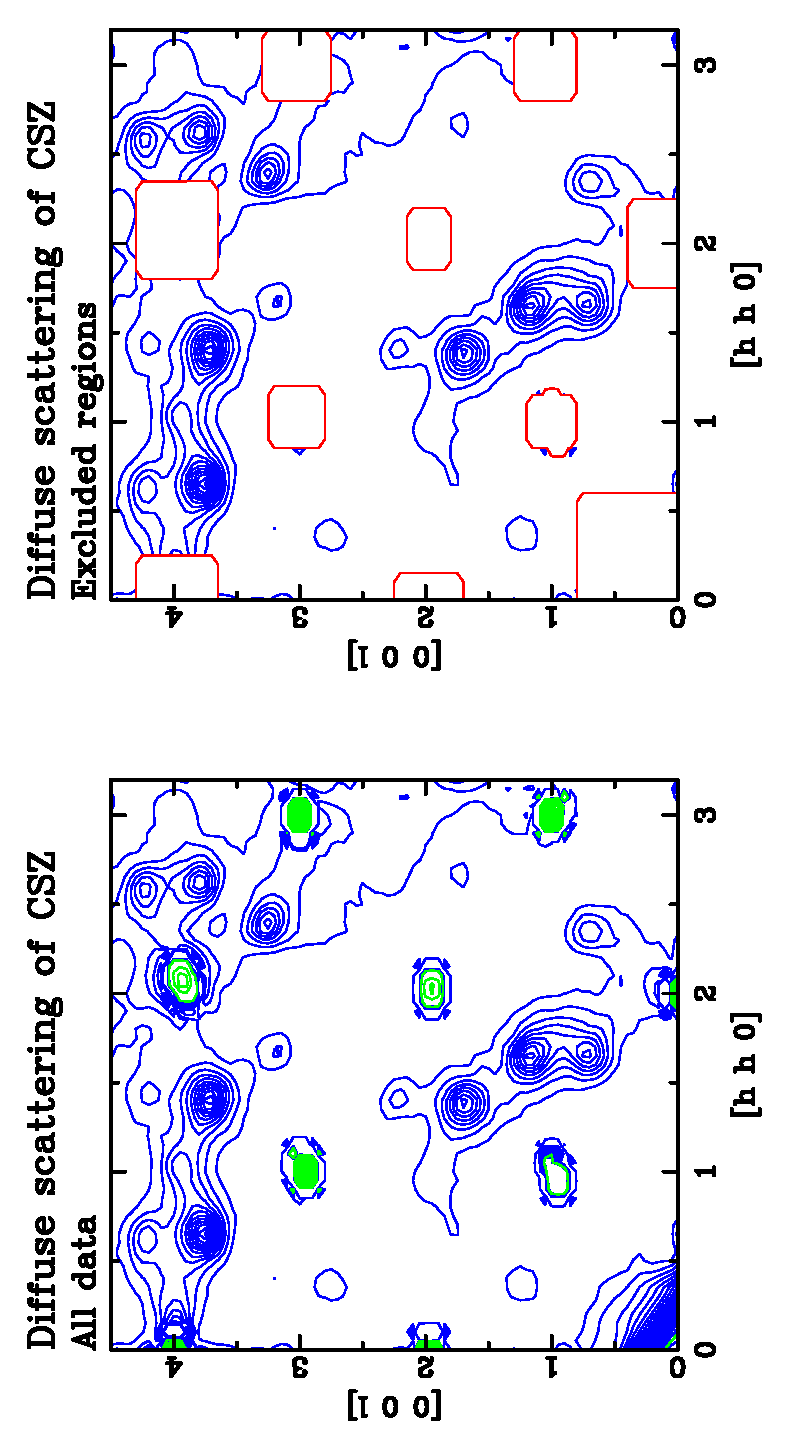
\includegraphics[scale=0.6, angle=270.0]{pl2.1.eps}
   \caption{Usage of excluded regions for 2D files}
   \label{pl2-fig1}
\end{figure}

The second more general 2D file format is the PGM (portable graymap)
format which is defined as part of the  PNM format Jef Poskanzer.
Various programs are capable of reading PNM files and the {\it
pnmplus-package} is a freely available collection of tools and
conversion programs from PNM to virtually any other graphics format.
{\it KUPLOT} only supports ASCII PGM files which are defined as
follows:

\begin{MacVerbatim}
    1      P2
    2      nx ny
    3      255
    4ff    z z z z z
\end{MacVerbatim}

The code {\it P2} in the first line identifies the file as ASCII PGM
format. The dimensions $nx$ and $ny$ of the data set are given in
the next line. The PGM format is an integer bitmap and the number in
line 3 gives the maximum depth (here 255 or 8 bit). Although the PGM
format is generally not restricted to 8 bit resolution, it was found
that many programs are not capable of reading PNM files with a
larger resolution. Comments can be included in the file starting
with a \# as first character. The actual data are integer values
written row by row starting (in contrast to NIPL files) from the top
left corner. Besides being limited to integer values ranging from $0
\rightarrow 255$, the PGM file format does not contain any
information about the $x$ and $y$ limits and {\it KUPLOT} sets x-
and y-values to the pixel number. However, the x- and y-values might
be manipulated (see chapter \ref{mat}) and the file can be saved in
NIPL format (see section \ref{2d-save}), thus allowing the
conversion of PGM files to NIPL files and {\it vice versa}.\par

The PGM and NIPL files are restricted to data points being on a
equidistant rectangular grid. The file format 'zz' can be used to
read any data file containing the data points $(x_{i}, y_{i},
z_{i})$ on a separate line. This is practically the extension of the
'xy' file format. However, {\it KUPLOT} can internally only work
with z-values lying on a rectangular equidistant grid. Thus the read
data points are binned to a grid size defined by $\Delta x$ and
$\Delta y$ given as additional parameters to the {\it load} command.
Each resulting grid point contains the average of all data points
within the file that fall within the area of the specific grid
point. If the specified grid size is too small, the resulting plot
will contain empty grid points. The following command reads the XYZ
file {\it test.xyz} and bins it to a grid size of $\Delta x = \Delta
y = 0.05$:

\begin{MacVerbatim}
    load zz,test.xyz,0.05,0.05
\end{MacVerbatim}

This file format can also be used to rebin data sets to a broader grid
by saving the NIPL (or PGM) file as XYZ file and rereading the file
with the new desired grid size. \par

The file format {\tt de} (for density) works similar to the
previously discussed {\tt zz} format but rather than averaging the
z-values in each grid point, the resulting z-value is the number of
points $(x_{i}, y_{i})$ falling within the corresponding grid volume
which is defined as before by the additional parameters $\Delta x$
and $\Delta y$. The program reads the first two real numbers in each
line as x- and y-value. For example {\it DISCUS} can export the atom
positions of all atoms without the translational part, i.e. all
atoms are in one unit cell. The resulting file can be read using the
{\tt cr} format resulting in a marker for each atom. Alternatively
the same file (since the first two numbers are $x$ and $y$) can be
read using the 'de' format which will result in a density plot which
can be displayed either using contour lines or a bitmap.

%------------------------------------------------------------------------

\section{Customizing the plot \label{2d-change}}

The command {\tt hart} selects the usage of contour lines, bitmaps
or both and is discussed in the next section. Here we want to
concentrate on commands used to change contour lines. The base
level, the interval and the number of contour line levels are
defined using the command {\tt hlin}:

\footnotesize
\begin{MacVerbatim}
    hlin 1,100,50,10
    hlin 2,10,10,9,%
\end{MacVerbatim}
\normalsize

{\it KUPLOT} supports multiple sets of contour lines, e.g.  one set
at low levels to display diffuse scattering and one set at higher
levels with a different spacing for the stronger Bragg peaks.  Each
set can be plotted in a different color.  The two example commands
above illustrate the {\tt hlin} command.  The first command sets the
values for contour line set 1.  The contours start at a value of 100
and increase in steps of 50.  A total of 10 contour levels is drawn,
e.g.  the highest level corresponds to 600. The second {\tt hlin}
commands sets values for the second contour line set, but the
additional parameter '\%' indicates, that the numbers are taken as
percentage of $\Delta z = zmax - zmin$ of all loaded data sets
rather than absolute z-values.  In our example the base level is
10\% of $\Delta z$, the contour lines are stepped in 10\% intervals
and 9 levels are plotted. Thus the highest level corresponds to
100\%.  The command {\tt hpak} determines how many contour line sets
are actually plotted.  The default is the usage of all sets defined
by the {\tt hlin} command.  Color and line type for the individual
contour line sets can be changed using the commands {\tt hcol} and
{\tt htyp}.

\begin{figure}[!tbhp]
   \centering
   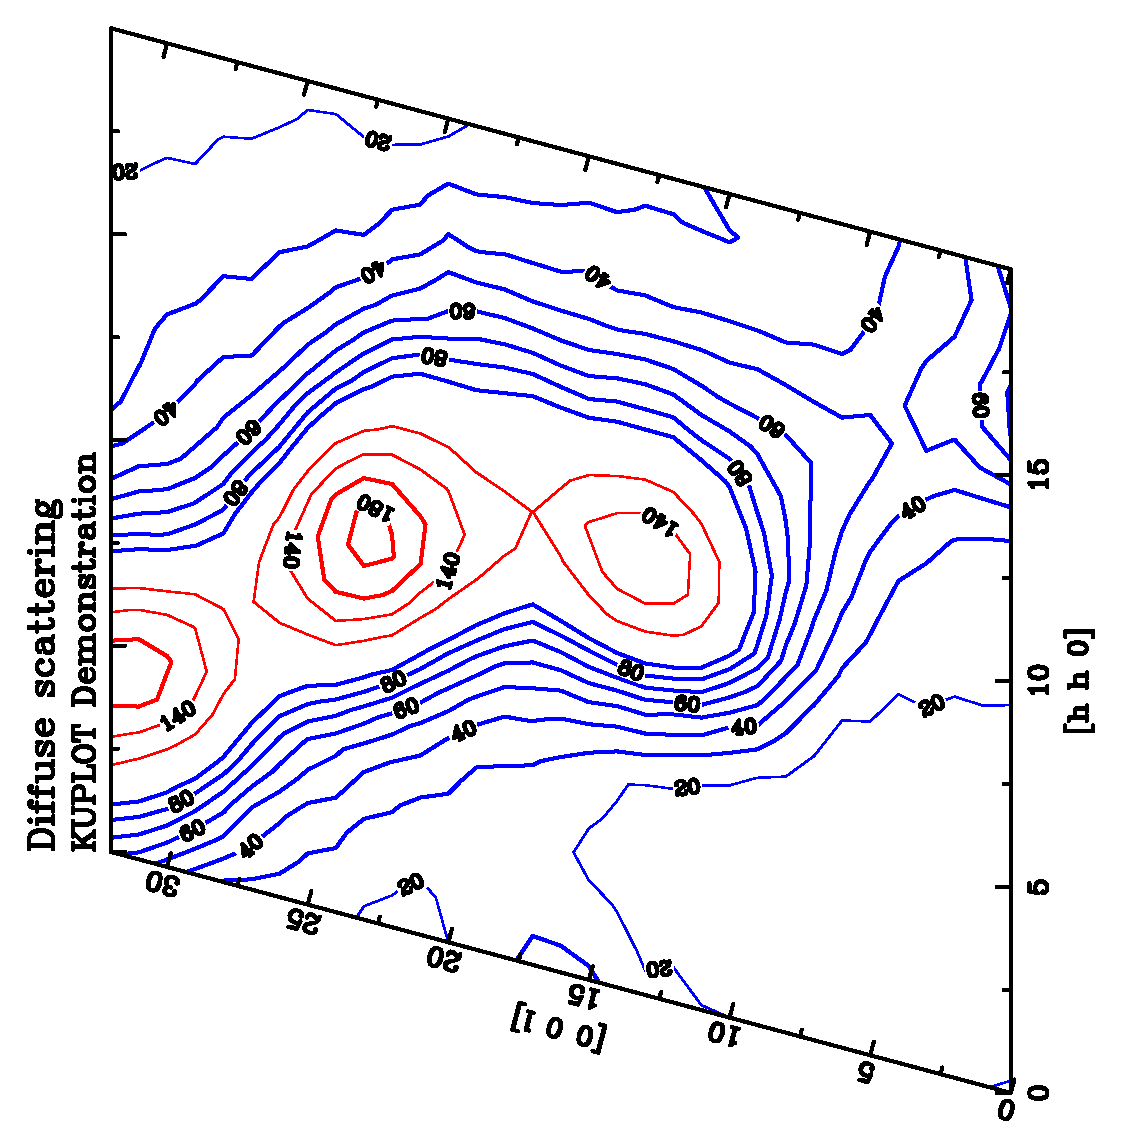
\includegraphics[scale=0.5, angle=270.0]{pl2.2.eps}
   \caption{Customizing contour plots}
   \label{pl2-fig2}
\end{figure}

Sometimes a specific aspect ratio of the x- and y-axis or a specific
angle between the two axis is required to obtain a non distorted
picture of the data.  {\it KUPLOT} allows the user to specify an
aspect ration using the {\tt aver} command.  As default {\it KUPLOT}
determines the aspect ratio is such a way, that the resulting plot
is as large as possible.  This default can be restored by entering
the command {\tt aver} without further parameters. Alternatively,
the desired ratio can be given as parameter to the {\tt aver}
command. In Figure \ref{pl2-fig2} we show an example of a contour
plot illustrating some of the features discussed above. The commands
used to create the contour lines shown are listed below:

\begin{MacVerbatim}
      1  aver 0.707
      2  angl 75.0
      3  #
      4  hlin 1, 10,10, 9
      5  hlin 2,120,20,10
      6  hcol 1,1,3
      7  hcol 1,2,1
      8  hlab 1,2
\end{MacVerbatim}

In line 1 we set the aspect ratio of the x- and y-axis to
$1/\sqrt{2} \approx 0.707$ and the angle between the axes to a value
of 75$^{\circ}$ (line 2). In lines 4--5 we define two contour line
packages, the first one giving contour lines at values of $z_{c} =
10, 20, ..., 100$ the second one at values $z_{c} = 120, 140, ...,
320$. In line 6 the color for the first contour package for data set
one is set to pen 3 (blue). Next the color for the second package
for the same data set is set to pen 1 (red). Finally the labeling of
contour lines for data set one is enabled. The second parameter in
line 8 specifies that every second contour line starting from the
base line is labeled. As always, check the online help for more
detailed information on the commands used.

%------------------------------------------------------------------------

\section{Using bitmaps \label{2d-bitmap}}

The command controlling the appearance of a 2D plot is {\tt hart}.
Its first parameter determines the data set, the second parameter
the type of plot. To use only contour lines set the second parameter
to 1, for bitmap display use 2 and to have both a bitmap and contour
lines set the second parameter of the {\tt hart} command to 3. In
Figure \ref{pl2-fig3} we can see the same plot using just a bitmap
on the bottom and using additional contour lines on the top. The
wedge showing the $z$ range of the bitmap colors is activated by
setting a label for the z-axis using the command {\tt achz}. \par

\begin{figure}[!tbhp]
   \centering
   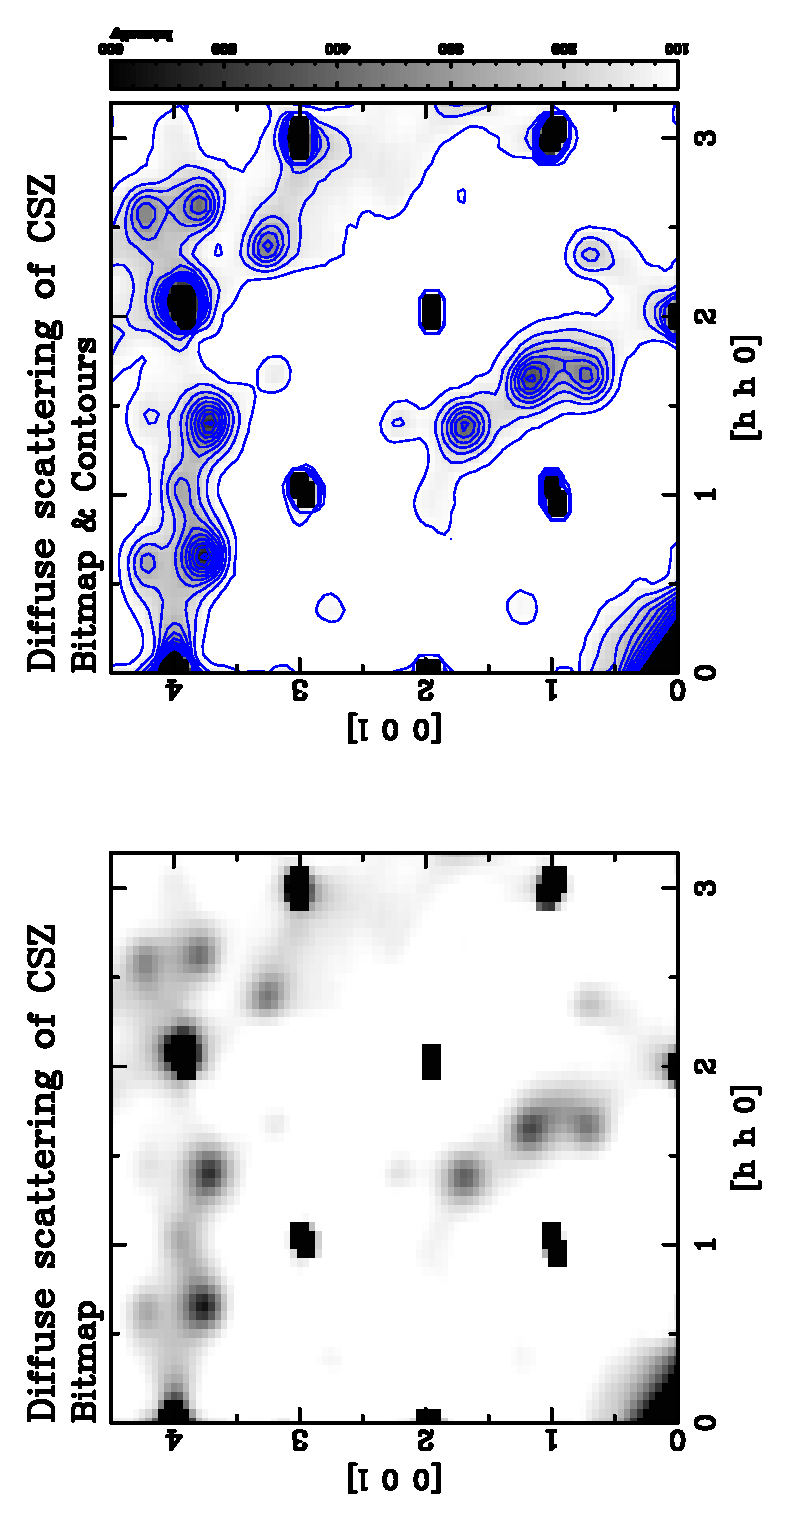
\includegraphics[scale=0.6, angle=270.0]{pl2.3.eps}
   \caption{Example for bitmap plots}
   \label{pl2-fig3}
\end{figure}

The bitmaps used by {\it KUPLOT} have 240 color entries, the
remaining 16 colors are reserved for other functions. The z-range to
be converted to those 240 colors is determined by the minimal and
maximal contour level for the first set defined by the command {\tt
hlin}. Subsequently the bitmap color range and the contour levels
are the same for the first set of contour levels. In some cases one
might want to create a plot where the bitmap and the contour lines
have different ranges. This can be done like in the following
example:

\begin{MacVerbatim}
    hlin 1,0,50,1,%
    hlin 2,0,5,20,%
    htyp 1,0
    htyp 2,1
\end{MacVerbatim}

The levels set by the first {\tt hlin} command determine the z-range
used to create the bitmap, i.e. 0\% to 50\% of the z-range. We do
this in a single step since only the maxima are used to determine
the bitmap. The second {\tt hlin} command sets the contour lines we
actually want to plot on top of the bitmap. In order to suppress the
first set of contour lines we set the line type for set 1 to 0, i.e.
no line using the first {\tt htyp} command. The line type for the
second contour set is set to 1, i.e. solid line, as done in the last
line of the example above. \par

{\it KUPLOT} has three default color maps used to display bitmaps.
The map is selected by the command {\tt cmap}. For a description of
the different color maps refer to the online help. The selected map
for the examples displayed in Figure \ref{pl2-fig3} is {\tt gray}.
The command {\tt cmap} is also used to save or read a color map from
a file. Additionally the current color map can be altered using the
variable {\it cmap}. For details about the usage of variables see
the section {\tt Varialse} in the general package manual 
\href{./package\_man.pdf}{DISCUS package}.

%------------------------------------------------------------------------

\section{Saving data \label{2d-save}}

\begin{figure}[!t]
   \centering
   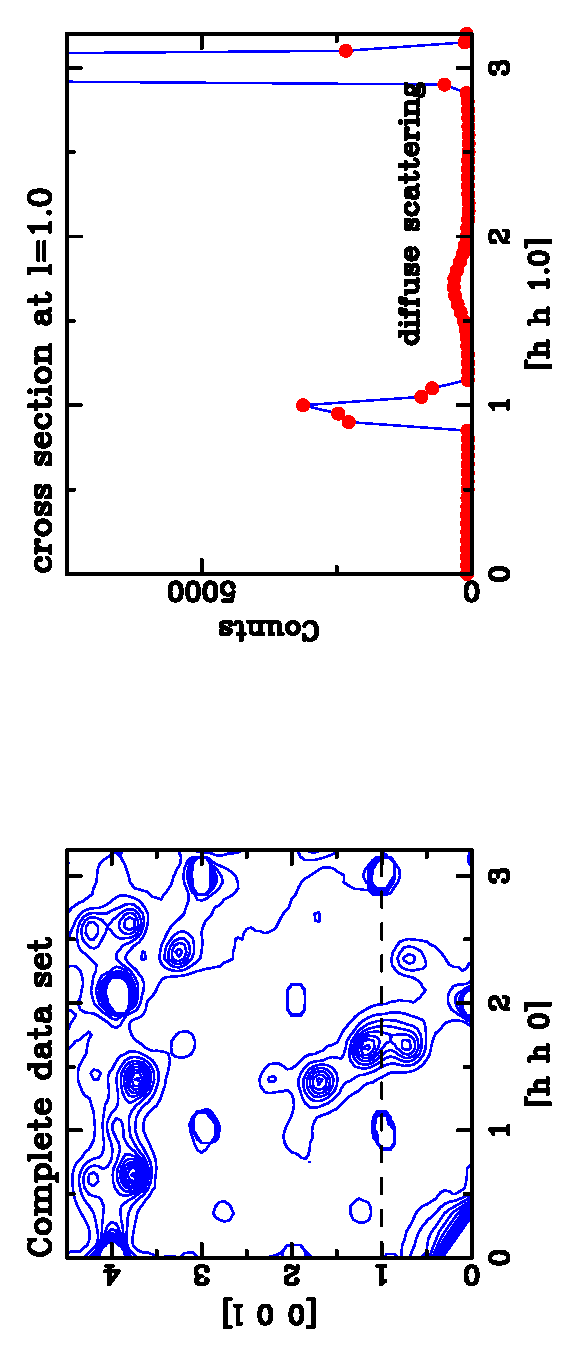
\includegraphics[scale=0.65, angle=270.0]{pl2.4.eps}
   \caption{Extracting data from 2D data sets}
   \label{pl2-fig4}
\end{figure}

In contrast to 1D data where we could mainly save a given data set
in the {\tt xy} format, there are several options to extract and
save data from a 2D data set. As described in section \ref{1d-save},
the first step is to enter the save sub level using the command {\tt
ksav} followed by the number of the data set to be saved. As before
the output filename is set by the command {\tt outfile} and the
saving process is started via {\tt run}. However, there are now many
more possible settings for the {\tt form} command.

\begin{table}[!b]
\centering
\begin{tabularx}{\textwidth}{|p{15mm}|p{45mm}|X|}
  \hline
  {\bf Format} & {\bf Parameters} & {\bf Description} \\
  \hline\hline
    ni & [x1,x2,y1,y2] & Nipl file, given area \\
    pg & [x1,x2,y1,y2] & PGM file (ASCII), given area \\
    gn & [x1,x2,y1,y2] & XYZ file (gnuplot), given area \\
  \hline
    sx & y-value       & Cross section $\|$ x at y-value \\
    sy & x-value       & Cross section $\|$ y at x-value \\
    mx & i             & Cross section $\|$ x through maximum \#i \\
    my & i             & Cross section $\|$ y through maximum \#i \\
    sk & ik            & Cross section along xy of data set ik \\
    sl & x1,y1,x2,y2,n & Cross section from x1,y1 to x2,y2 with n points \\
  \hline
\end{tabularx}
\caption{\label{pl2-tab2}Save options for 2D data sets}
\end{table}

The first three of those formats listed in Table \ref{pl2-tab2} save
the data set or a subsection as 2D data set either in NIPL, PGM or
XYZ format. As before the area that is saved is determined by the
current size of the plot window determined by the command {\tt
skal}. Alternatively the x-limits $x1$ and $x2$ and y-limits $y1$
and $y2$ can be specified as additional parameters to the 'form'
command. Note that when using PGM as output format, the z-values are
converted to integer and should range from $0 \rightarrow 255$. The
command 'thresh' allows to control how the z-values are converted to
this range. The other formats in Table \ref{pl2-tab2} are used to
extract a cross section from the 2D data set. The created output
file is a normal {\tt xy} file. The parameters {\tt sx} and {\tt sy}
extract a cross section parallel to the x- or y-axis at the given y-
or x-value (see example below). Rather than specifying these y- or
x-values, the corresponding coordinates of maximum $i$ determined by
the command {\tt smax} (see section \ref{mat}) can be used ({\tt mx}
or {\tt my}). The command above will extract the z-values at the
corresponding grid points. The last two options can extract data
from any value of $x$ and $y$ by interpolation. The format {\tt sk}
will use the coordinates $x$ and $y$ from data set (1D) number {\tt
ik} to determine the z-values to be extracted whereas {\tt sl} will
extract $n$ points along a straight line defined by the points
$(x1,y1)$ and $(x2,y2)$. \par

A simple example how to extract a cross section is show in Figure
\ref{pl2-fig4}. The original data set is shown on the left. The
cross section parallel x (or [hh0]) at y (or l) equals 1.0 is
marked by a dashed line. The resulting 1D plot of the cross
section is shown on the right panel of the figure. The
corresponding commands to create the data file shown at the top is
listed below:

\begin{MacVerbatim}
     1  ksav 1
     2  outfile test.cut
     3  form sx,1.0
     4  run
\end{MacVerbatim}

In line 1 we enter the save sub level. In our example the data set to
be used is data set number one. The output filename is set to {\it
test.cut} (line 2) and the format is set to {\tt sx}, i.e. cross
section parallel to $x$ at $y=1.0$ (line 3). Finally the data file
is written after the command {\tt run} is entered (line 4).


%------------------------------------------------------------------------
